\documentclass[pdflatex,sn-mathphys-num]{sn-jnl}% Math and Physical Sciences Numbered



\input{generalconfig.tex}



\begin{document}



\title[Article Title]{TFT Screen Library (SPI Version)}


\author*[1,2]{\fnm{Contreras R} \sur{Orlando}}\email{\{al348390,al464376\}@edu.uaa.mx}

\author*[1,2]{\fnm{Lara H} \sur{Kevin}}


\affil[3]{\orgdiv{Department of Electronic Systems}, \orgname{UAA}, \orgaddress{\street{Av. Universidad 940}, \city{Aguascalientes}, \postcode{20131}, \state{Aguascalientes}, \country{México}}}



%%==================================%%

%% Sample for unstructured abstract %%

%%==================================%%



\abstract{The objective of this TFT$\_$LCD screen driver is implement an easy way to show info on a screen. This is very useful in embedded systems applications, like show images, text, or anything that requires a screen.}

%% me dices si ocupas ayuda con algo ire a desyunar oki probecho

%%================================%%

%% Sample for structured abstract %%

%%================================%%



\keywords{ARM, C++, Driver, TFT Screen.}



%%\pacs[JEL Classification]{D8, H51}



%%\pacs[MSC Classification]{35A01, 65L10, 65L12, 65L20, 65L70}



\maketitle





\section{Introduction}\label{sec1}

Communication protocols are very useful in a lot of tech applications; all computers, micro controllers, and every circuit with a processor need communication protocols to send or receive I/O data and control external peripherals, some of the most used protocols are SPI. Using this application, the ST7735 TFT screen is a device able to print pixels on a point-matrix, sending via SPI the column and row address to set the internal screen pointer on the pixel that we want to turn on, subsequently we send the color data of this pixel in the color format RGB565.  





\subsection{RGB565}

The RGB565 color format is a 16-bit representation of colors, where 5 bits are used for red, 6 bits for green, and 5 bits for blue. This allows for a total of 65,536 different colors. The format is structured as follows:

\begin{figure}[!h]

    \centering

    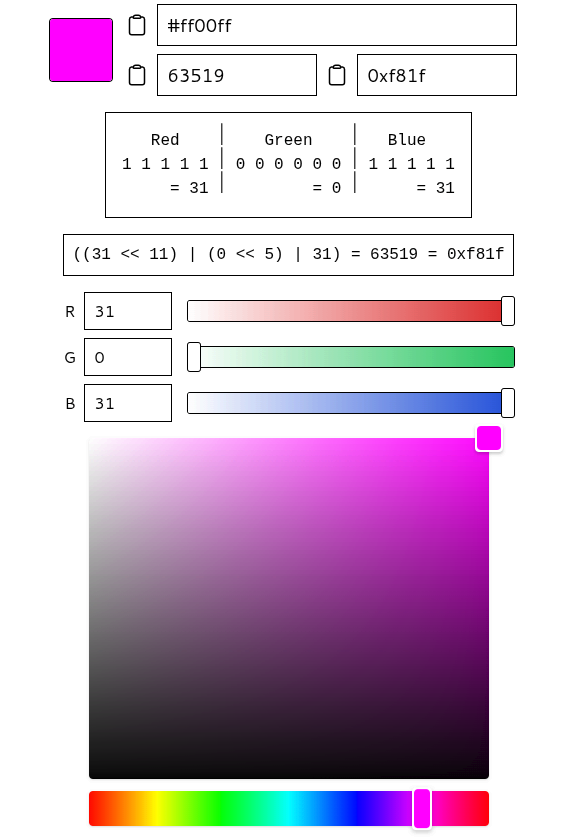
\includegraphics[width=0.5\linewidth]{MIPI/RGB565.png}

    \caption{RGB Format}

    \label{fig:rgb565}

\end{figure}



Here we got the pink color on RGB565 format (0xF81F), the red color (0xF800), the green color (0x07E0), and the blue color (0x001F), while on RGB888 the pink color is (0xFF00FF), the red color (0xFF0000), the green color (0x00FF00), and the blue color (0x0000FF). 

Therefore we could get the conversion from RGB888 to RGB565 using the following formula:



\begin{figure}[!h]

    \centering

    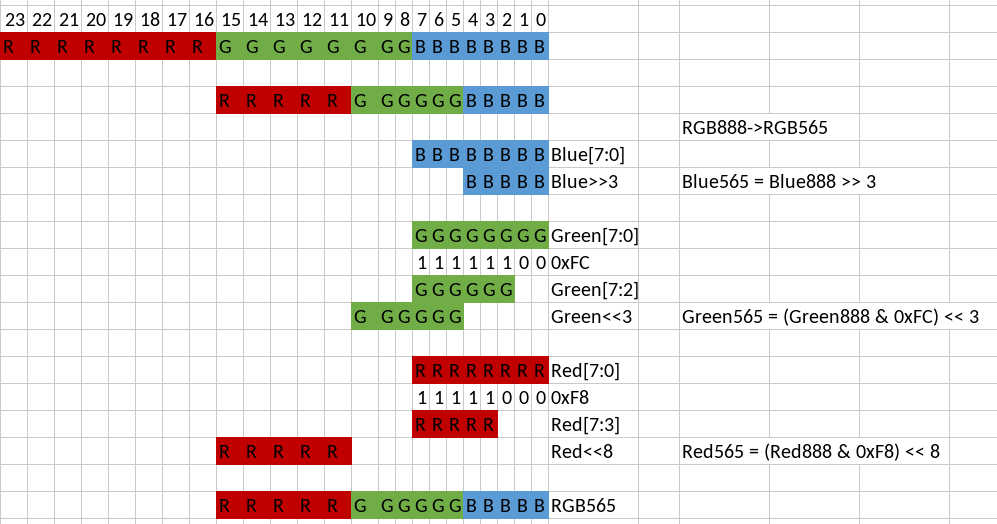
\includegraphics[width=0.8\linewidth]{MIPI/RGB565Conv.png}

    \caption{RGB565 Conversion Formula}

    \label{fig:rgb565conv}

\end{figure}

\begin{equation}
RGB565 = ((R \& 0xF8) << 8) | ((G \& 0xFC) << 3) | (B >> 3)
\end{equation}

If we didnt had the colors itselfs, we could use the following formula to get the RGB565 color from the RGB888 color:

\begin{equation}
RGB565 = (((RGB888 \& 0xf80000)>>8) + ((RGB888\&0xfc00)>>5) + ((RGB888\&0xf8)>>3));
\end{equation}

\begin{figure}

    \centering

    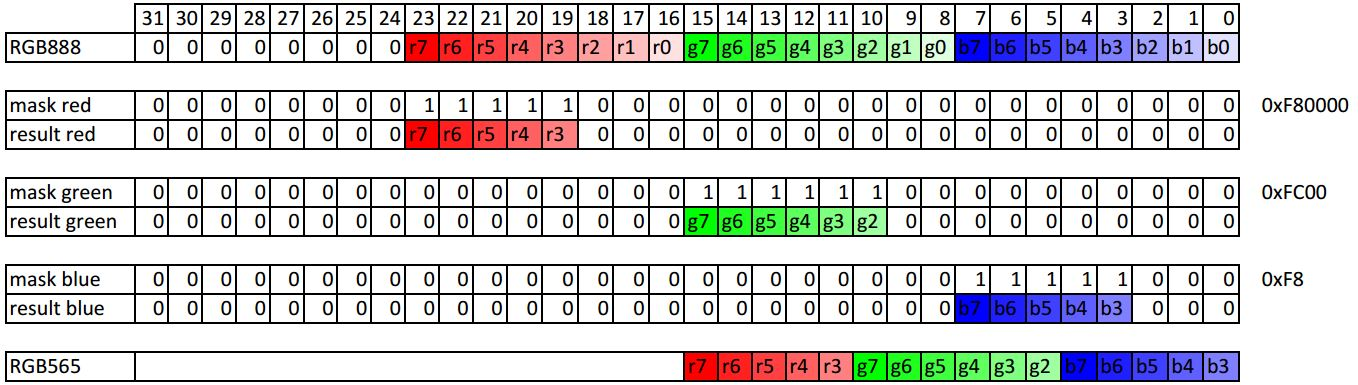
\includegraphics[width=0.8\linewidth]{MIPI/RGBConversion.png}

    \caption{RGB Color Conversion Process}

    \label{fig:rgbconversion}

\end{figure}

%https://barth-dev.de/about-rgb565-and-how-to-convert-into-it/

%https://chipsncode.com/tools/rgb565-colour-reference/

%https://rgbcolorpicker.com/565



\section{ST7735}



\begin{figure}

    \centering

    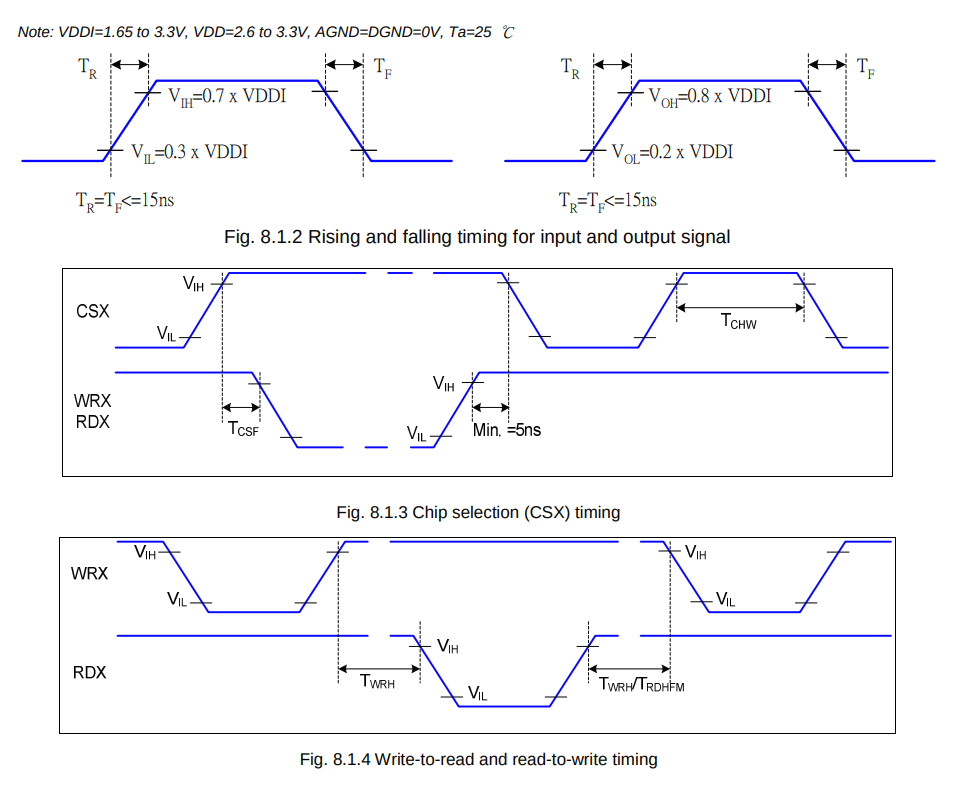
\includegraphics[width=0.5\linewidth]{MIPI/Considerations.png}

    \caption{ST7735 Interface Considerations}

    \label{fig:Cons}

\end{figure}



The screen ST7735 handles two interfaces

\begin{itemize}

    \item 3-Line/9-bit Serial interface (CS (Chip Select), SCL (Signal Clock), SDA (Serial Data Input/Output)) 

    \item 4-Line/8-bit Serial interface (CS (Chip Select), SCL (Signal Clock), SDA (Serial Data Input/Output), D/CX (Data/Command Flag))

\end{itemize}

We could switch between them with s
$$
\begin{cases}
    SPI4W = 0 & \text{(3-Line Serial interface)} \\
    SPI4W = 1 & \text{(4-Line Serial interface)}
\end{cases}
$$
\begin{figure}[!h]

    \centering

    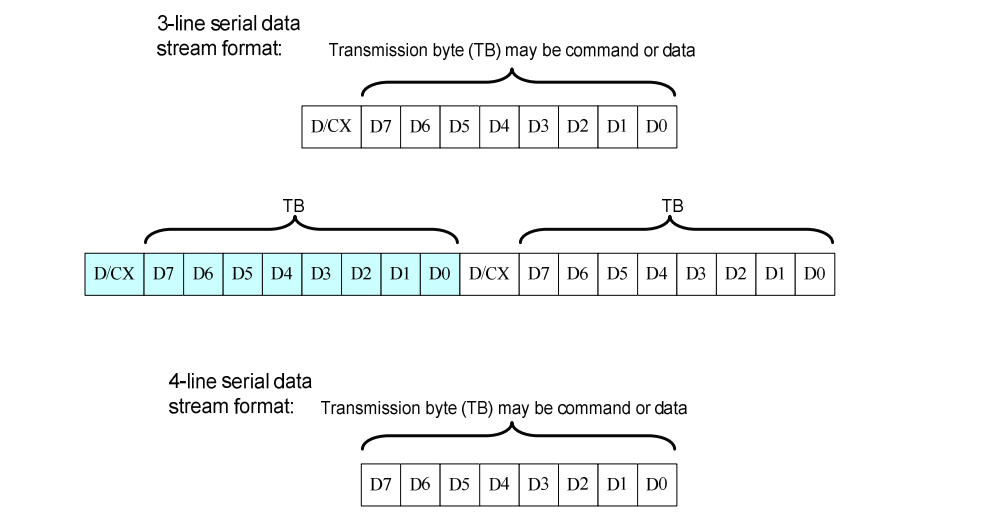
\includegraphics[width=0.7\linewidth]{MIPI/3Lines.png}

    \caption{3-Line and 4-Line Serial Interface}

    \label{fig:3lines}

\end{figure}


\subsection{Time and Voltage Considerations}
Should be considered the following specifications for the ST7735 screen, the voltage levels and the time of the signals, as shown in figure \ref{fig:Cons}. We take the VDDI voltage as 3.3V same as VDD.

\begin{figure}[!h]
    \centering
    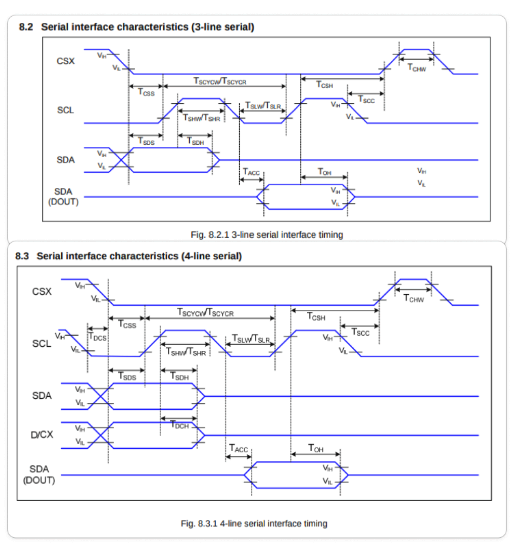
\includegraphics[width=0.5\linewidth]{MIPI/Timing.png}
    \caption{Timing Constraints}
    \label{fig:timing}
\end{figure}

\begin{table}[!h]
\centering
\caption{4-line Serial Interface Characteristics}
\label{tab:serial_interface}
\begin{tabular}{|l|l|l|c|c|c|}
\hline
\textbf{Signal} & \textbf{Symbol} & \textbf{Parameter} & \textbf{MIN} & \textbf{MAX} & \textbf{Unit} \\ \hline
\multirow{5}{*}{CSX} & TCSS & Chip select setup time (write) & 15 & & ns \\ 
                     & TCSH & Chip select hold time (write) & 15 & & ns \\ 
                     & TCSS & Chip select setup time (read) & 60 & & ns \\ 
                     & TSCC & Chip select hold time (read) & 65 & & ns \\ 
                     & TCHW & Chip select ``H'' pulse width & 40 & & ns \\ \hline
\multirow{6}{*}{SCL} & TSCYCW & Serial clock cycle (Write) & 66 & & ns \\ 
                     & TSHW & SCL ``H'' pulse width (Write) & 30 & & ns \\ 
                     & TSLW & SCL ``L'' pulse width (Write) & 30 & & ns \\ 
                     & TSCYCR & Serial clock cycle (Read) & 150 & & ns \\ 
                     & TSHR & SCL ``H'' pulse width (Read) & 60 & & ns \\ 
                     & TSLR & SCL ``L'' pulse width (Read) & 60 & & ns \\ \hline
\multirow{2}{*}{D/CX} & TDCS & D/CX setup time & & 0 & ns \\ 
                      & TDCH & D/CX hold time & 10 & & ns \\ \hline
\multirow{4}{*}{\begin{tabular}[c]{@{}l@{}}SDA\\ (DIN)\\ (DOUT)\end{tabular}} 
                     & TSDS & Data setup time & 10 & & ns \\ 
                     & TSDH & Data hold time & 10 & & ns \\ 
                     & TACC & Access time & 10 & 50 & ns \\ 
                     & TOH & Output disable time & & 50 & ns \\ \hline
\end{tabular}
\end{table}

\begin{table}[!h]
\centering
\caption{Parallel 8080-Series MCU Interface Characteristics}
\label{tab:parallel_8080_interface}
\begin{tabular}{|l|l|l|c|c|c|}
\hline
\textbf{Signal} & \textbf{Symbol} & \textbf{Parameter} & \textbf{MIN} & \textbf{MAX} & \textbf{Unit} \\ \hline
\multirow{2}{*}{D/CX} & AST & Address setup time & 0 & & ns \\ 
                      & AHT & Address hold time (Write/Read) & 10 & & ns \\ \hline
\multirow{3}{*}{CSX} & CHW & Chip select ``H'' pulse width & 0 & & ns \\ 
                     & CSXN & Chip select setup time (Write) & 15 & & ns \\ 
                     & CSRN & Chip select setup time (Read ID) & 45 & & ns \\ \hline
\multirow{3}{*}{WRX} & TWC & Write cycle & 66 & & ns \\ 
                     & WRH & Write Control ``H'' pulse width & 15 & & ns \\ 
                     & WRL & Write Control ``L'' pulse width & 15 & & ns \\ \hline
\multirow{3}{*}{RDX (ID)} & TRCFM & Read cycle (FM) & 450 & & ns \\ 
                         & RDHFM & Read Control ``H'' pulse width (FM) & 90 & & ns \\ 
                         & RDLFM & Read Control ``L'' pulse width (FM) & 355 & & ns \\ \hline
\multirow{4}{*}{D[17:0]} & DST & Data setup time & 10 & & ns \\ 
                         & DHT & Data hold time & 10 & & ns \\ 
                         & RAT & Read access time (FM) & & 340 & ns \\ 
                         & ODH & Output disable time & 20 & 80 & ns \\ \hline
\end{tabular}
\end{table}



\section{Description}

The library for the ST7735-based TFT display provides a simple and efficient interface for handling graphics through the SPI communication protocol. 



This library abstracts the complexity of the command sequences and internal operation of the ST7735, offering intuitive functions to initialize the display, print color rectangles,fill the creen with one color, draw pixels, and test the colors on the screen, each one integrated on a 4 simple function to use:



Screen1.FillScreen(color).



Screen1.FillRectangle(posx, posy, width, height, color).



Screen1.DrawPixel(posyx, posy, color).
test(void);

\subsection{Gamma Adjustments (Positive and Negative Polarity)}
The ST7735 controller features highly customizable Gamma Correction registers (\texttt{ST7735\_GMCTRP1} for positive polarity and \texttt{ST7735\_GMCTRN1} for negative polarity). In Liquid Crystal Displays (LCDs), gamma correction is not merely a software tool for contrast styling, but a critical hardware requirement to compensate for the non-linear electro-optical transfer characteristics of the liquid crystal layer.

\subsubsection{Understanding Polarity in Gamma Control}
Liquid crystal molecules are sensitive to the root-mean-square (RMS) value of an electric field. If a constant DC voltage is applied continuously in a single direction across the liquid crystal cells, it causes ion polarization and chemical degradation, permanently damaging the screen (a phenomenon known as \textit{image sticking} or LCD burn-in). 

To prevent this, TFT displays use an Alternating Current (AC) driving method where the polarity of the voltage applied to each pixel is inverted periodically (typically per frame or per line) relative to a common reference voltage ($V_{COM}$). 
\begin{itemize}
    \item \textbf{Positive Polarity (\texttt{GMCTRP1}):} Defines the voltage-to-grayscale mapping curve when the pixel voltage is higher than $V_{COM}$.
    \item \textbf{Negative Polarity (\texttt{GMCTRN1}):} Defines the voltage-to-grayscale mapping curve when the pixel voltage is lower than $V_{COM}$.
\end{itemize}

Because the physical behavior of liquid crystals can vary slightly depending on whether the charge is positive or negative, independent 16-argument register arrays are required to guarantee that a specific grayscale value outputs the exact same optical luminance in both polarities, preventing screen flickering.

\subsubsection{Determination of Gamma Values}
The 16 hexadecimal parameters passed to each gamma register block represent specific tap points along a digital-to-analog converter (DAC) voltage resistor ladder. These target points adjust key characteristics of the curve:
\begin{itemize}
    \item \textbf{Low-order parameters} alter the black levels and dark gray gradients.
    \item \textbf{Mid-order parameters} fine-tune the mid-tones and linearity of the color distribution.
    \item \textbf{High-order parameters} determine the peak white saturation levels.
\end{itemize}

In practical driver development, these values are \textbf{empirically determined by the display module manufacturer}. The screen vendor utilizes specialized optical instrumentation (such as colorimeters and spectrophotometers) to measure the luminance response across the grayscale spectrum on a bare glass panel panel sample. 

The factory engineers then calculate the exact DAC voltage offsets required to match standard target curves (typically a Gamma 2.2 profile, which matches human visual perception). The resulting magic numbers—such as the ones embedded in our \texttt{init\_cmd[]} array—are hardcoded into the initialization routine to ensure accurate color reproduction, stable grayscale transitions, and identical luminance across both positive and negative driving cycles.

\section{Initialization Sequence}
The following array contains the configuration sequence for the ST7735R controller. To distinguish between commands and data control packets within the bare-metal driver, a \texttt{0x0100} prefix mask is applied to metadata parameters, while direct commands maintain their hardware definitions.

\begin{lstlisting}[
    language=C++,
    basicstyle=\ttfamily\small,
    keywordstyle=\color{blue},
    commentstyle=\color{gray},
    numbers=left,
    numberstyle=\tiny\color{gray},
    stepnumber=1,
    numbersep=8pt,
    frame=single,
    breaklines=true,
    tabsize=4,
    showstringspaces=false
]
uint16_t init_cmd[] = {
    // Init for 7735R, part 1 (red or green tab)
    ST7735_SWRESET, // 1: Software reset, 0 args, w/delay
    ST7735_SLPOUT , // 2: Out of sleep mode, 0 args, w/delay
    ST7735_FRMCTR1, // 3: Frame rate ctrl - normal mode, 3 args:
    0x0101,         //    Argument 1: RTNA setting
    0x012C,         //    Argument 2: FPA setting
    0x012D,         //    Argument 3: BPA setting. Rate = fosc/(1x2+40) * (LINE+2C+2D)
    ST7735_FRMCTR2, // 4: Frame rate control - idle mode, 3 args:
    0x0101,         //    Argument 1: RTNB setting
    0x012C,         //    Argument 2: FPB setting
    0x012D,         //    Argument 3: BPB setting. Rate = fosc/(1x2+40) * (LINE+2C+2D)
    ST7735_FRMCTR3, // 5: Frame rate ctrl - partial mode, 6 args:
    0x0101,         //    Argument 1: RTNC setting
    0x012C,         //    Argument 2: FPC setting
    0x012D,         //    Argument 3: BPC setting (Dot inversion mode)
    0x0101,         //    Argument 4: RTNC setting 
    0x012C,         //    Argument 5: FPC setting
    0x012D,         //    Argument 6: BPC setting (Line inversion mode)
    ST7735_INVCTR , // 6: Display inversion ctrl, 1 arg, no delay:
    0x0107,         //    Argument 1: No inversion (Line inversion on full/idle/partial)
    ST7735_PWCTR1 , // 7: Power control, 3 args, no delay:
    0x01A2,         //    Argument 1: GVDD setup
    0x0102,         //    Argument 2: VCI1 / VGH / VGL setup (-4.6V)
    0x0184,         //    Argument 3: Opamp bias selection (AUTO mode)
    ST7735_PWCTR2 , // 8: Power control, 1 arg, no delay:
    0x01C5,         //    Argument 1: VGH25 = 2.4C, VGSEL = -10, VGH = 3 * AVDD
    ST7735_PWCTR3 , // 9: Power control, 2 args, no delay:
    0x010A,         //    Argument 1: Opamp current small (Normal mode)
    0x0100,         //    Argument 2: Boost frequency (Normal mode)
    ST7735_PWCTR4 , // 10: Power control, 2 args, no delay:
    0x018A,         //    Argument 1: BCLK/2, Opamp current small & Medium low (Idle)
    0x012A,         //    Argument 2: Boost frequency (Idle mode)
    ST7735_PWCTR5 , // 11: Power control, 2 args, no delay:
    0x018A,         //    Argument 1: Opamp current and boost (Partial mode)
    0x01EE,         //    Argument 2: Boost frequency (Partial mode)
    ST7735_VMCTR1 , // 12: Power control, 1 arg, no delay:
    0x010E,         //    Argument 1: VCOM voltage setting
    ST7735_INVOFF , // 13: Don't invert display, no args, no delay
    ST7735_MADCTL , // 14: Memory access control (directions), 1 arg:
    ST7735_ROTATION,//    Argument 1: Row/Col address scan, bottom to top refresh
    ST7735_COLMOD , // 15: Set color mode, 1 arg, no delay:
    0x0105 ,        //    Argument 1: 16-bit color format (RGB565)
    ST7735_CASET  , // 16: Column addr set, 4 args, no delay:
    0x0100,         //    Argument 1: XSTART high byte
    0x0100,         //    Argument 2: XSTART low byte = 0
    0x0100,         //    Argument 3: XEND high byte
    0x017F,         //    Argument 4: XEND low byte = 127
    ST7735_RASET  , // 17: Row addr set, 4 args, no delay:
    0x0100,         //    Argument 1: YSTART high byte
    0x0100,         //    Argument 2: YSTART low byte = 0
    0x0100,         //    Argument 3: YEND high byte
    0x017F,         //    Argument 4: YEND low byte = 127
    ST7735_GMCTRP1, // 18: Gamma Adjustments (pos. polarity), 16 args, no delay:
    0x0102, 0x011c, 0x0107, 0x0112, // Arguments 1 to 4: Curve mapping
    0x0137, 0x0132, 0x0129, 0x012d, // Arguments 5 to 8: Curve mapping
    0x0129, 0x0125, 0x012B, 0x0139, // Arguments 9 to 12: Curve mapping
    0x0100, 0x0101, 0x0103, 0x0110, // Arguments 13 to 16: Curve mapping
    ST7735_GMCTRN1, // 19: Gamma Adjustments (neg. polarity), 16 args, no delay:
    0x0103, 0x011d, 0x0107, 0x0106, // Arguments 1 to 4: Curve mapping
    0x012E, 0x012C, 0x0129, 0x012D, // Arguments 5 to 8: Curve mapping
    0x012E, 0x012E, 0x0137, 0x013F, // Arguments 9 to 12: Curve mapping
    0x0100, 0x0100, 0x0102, 0x0110, // Arguments 13 to 16: Curve mapping
    ST7735_NORON  , // 20: Normal display on, no args, w/delay
    ST7735_DISPON   // 21: Main screen turn on, no args w/delay
};
\end{lstlisting}

\section{Purpose}

This library aims to support rapid development of visual interfaces, diagnostic screens, and real-time graphical outputs, offering a set of functions optimized for performance and compatibility with a wide range of microcontrollers. It is designed to serve both beginners and advanced users who require a practical and flexible tool to integrate TFT graphics into their projects.



\section{How to use properly}

This section explains how to integrate and use the ST7735 TFT driver and the oscilloscope demo on an STM32F446 MCU.



\subsection{Driver Initialization}

\begin{enumerate}

    \item Instantiate the driver object (constructor calls low-level \texttt{config()} for RCC/GPIO/SPI).

    \item Call \texttt{INIT\_FN()} once after reset to send the ST7735 init sequence.

    \item Clear or paint the screen using \texttt{FillScreen(color)}.

\end{enumerate}

Example:

\begin{verbatim}

TFT_ST7735 tft;

tft.INIT_FN();

tft.FillScreen(COLOR_BLACK);

\end{verbatim}



\subsection{Drawing Primitives}

\begin{itemize}

    \item Pixel: \verb|DrawPixel(x, y, color)|

    \item Rectangle: \verb|FillRectangle(x, y, w, h, color)| (auto clipping)

    \item Full screen: \verb|FillScreen(color)|

    \item Text: \verb|WriteChar(x, y, ch, font, fg, bg)| and \verb|WriteString(x, y, str, font, fg, bg)|

\end{itemize}

Colors use RGB565; predefined constants (\verb|COLOR_RED|, \verb|COLOR_BLUE|, etc.) live in the header.



\subsection{Oscilloscope Demo Flow}

Provided in \texttt{main\_osc.cpp}:

\begin{enumerate}

    \item Configure PLL and system clock via \texttt{conf\_osc()}.

    \item Enable and start continuous conversion on ADC1 channel at \texttt{PA0}.

    \item Initialize TFT and draw axes using rectangles.

    \item In loop: read \verb|ADC1->DR|, scale value (\verb|>>5|) to horizontal pixel range, increment vertical time index, plot with \verb|DrawPixel()|.

    \item When vertical index reaches bottom, clear plot region and restart for a scrolling effect.

\end{enumerate}



\subsection{Build Notes}

The code uses bare-metal register access (no HAL). Ensure your linker script and startup file match STM32F446. SPI baud is set to fPCLK/16. If the display shows nothing, verify wiring and that HSE/PLL configuration succeeds.



\subsection{Testing}

\begin{enumerate}

    \item Power the board and TFT (3.3V only).

    \item Flash firmware containing either \texttt{main\_tst.cpp} (color test) or \texttt{main\_osc.cpp} (oscilloscope).

    \item For oscilloscope: vary the analog input on PA0 (potentiometer or waveform source) and observe horizontal deflection of the cyan trace.

\end{enumerate}





\section{Diagram}

In figure \ref{fig:sq} the test circuit with the test code printing multiple rectangles, notice that the connections are in table \ref{tab:con}.



\begin{figure}[!h]

    \centering

    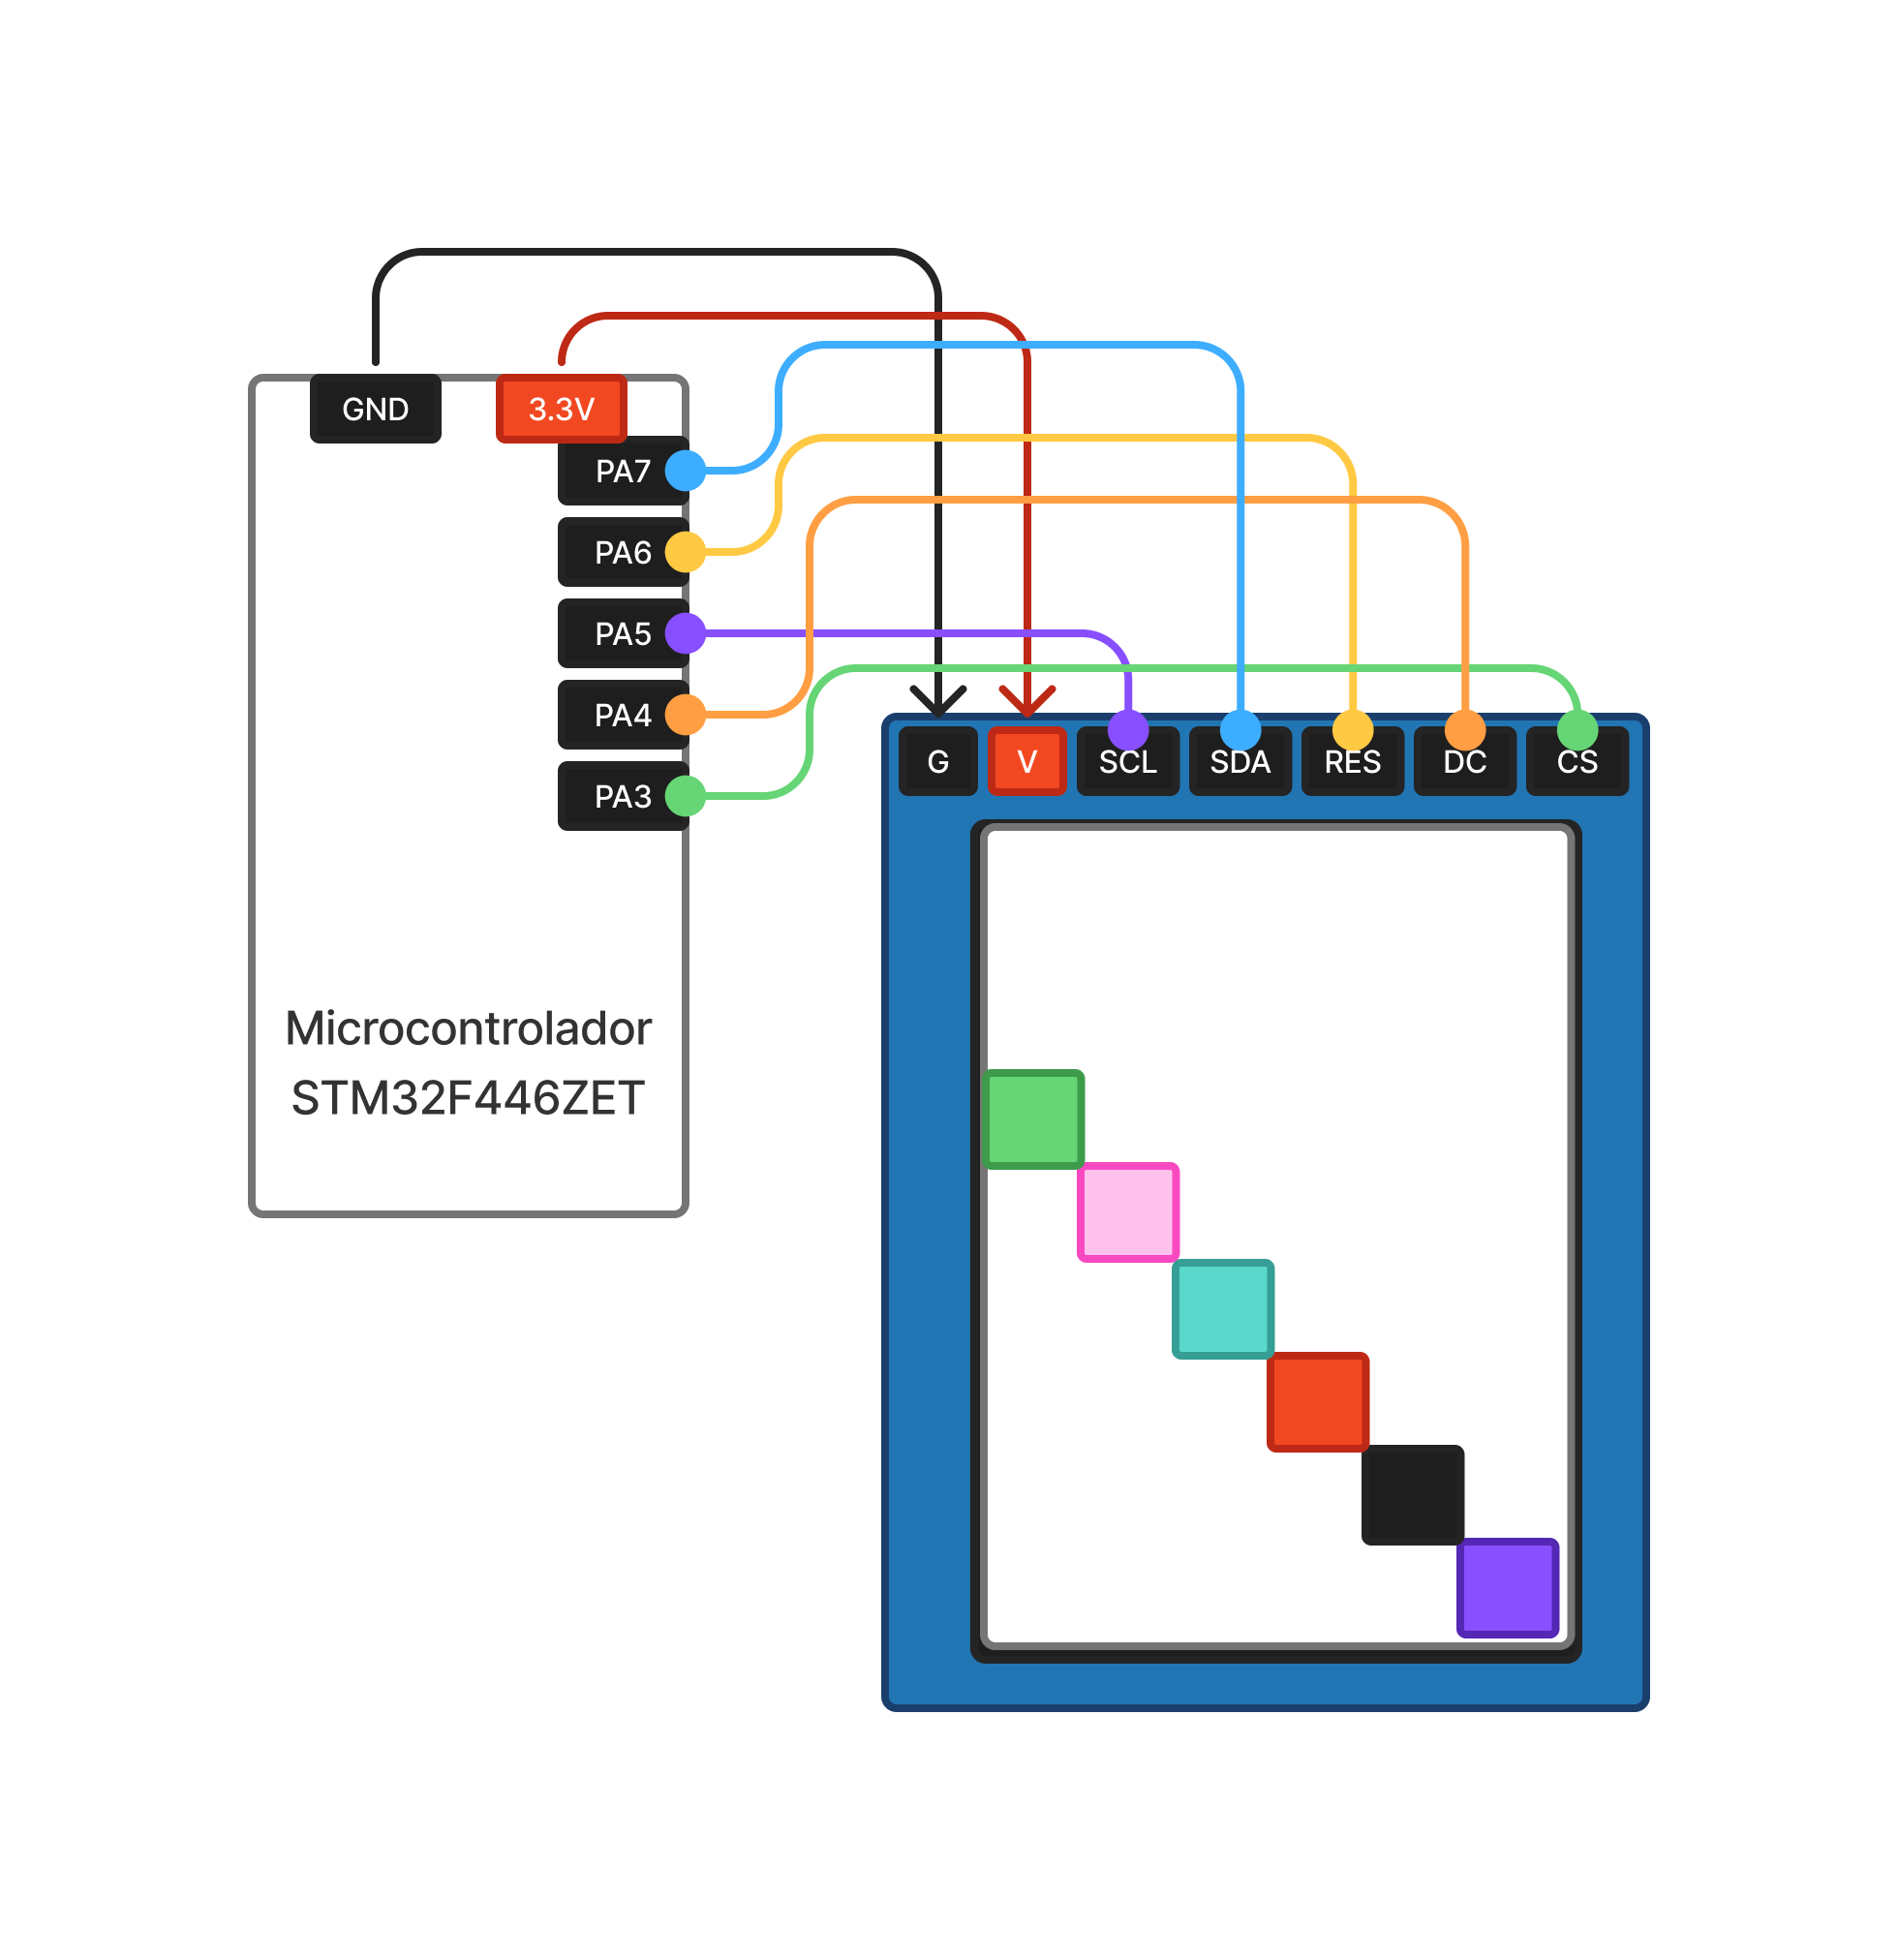
\includegraphics[width=0.5\linewidth]{MIPI/Esquematico.png}

    \caption{Schematic}

    \label{fig:sq}

\end{figure}



\begin{table}[!h]
\centering
\caption{TFT to STM32F446 Pin Connections}
\label{tab:con}
\begin{tabular}{|c|c|c|}

\hline TFT Pin & STM32F446 Pin & Purpose \\

\hline VCC & 3.3V & Power \\

GND & GND & Ground \\

SCK & PA5 & SPI1 SCK (AF5) \\

MOSI & PA7 & SPI1 MOSI (AF5) \\

CS & PA3 & Chip Select (GPIO) \\

DC & PA4 & Data/Command select (GPIO) \\

RST & PA6 & Hardware reset (GPIO) \\

\hline

\end{tabular}
\end{table}

Optional: connect a variable analog signal (e.g. potentiometer wiper) to \texttt{PA0} for the oscilloscope demo (ADC input).



\section{Limitations and Enhancements}

\subsection{Current Limitations}

\begin{itemize}

    \item \textbf{Polling SPI}: All transfers busy-wait; CPU cannot perform other tasks concurrently.

    \item \textbf{No DMA}: Large area fills and waveform plotting are slower than possible; higher CPU usage.

    \item \textbf{Fixed Rotation}: Only one memory access orientation initialized; no runtime rotation switching.

    \item \textbf{Limited Primitives}: Lines, circles, bitmaps, and sprites are not yet implemented.

    \item \textbf{No Text Clipping}: Long strings may draw off-screen without wrapping or truncation.

    \item \textbf{Oscilloscope Scaling}: Simple right-shift scaling (\verb|>>5|) reduces resolution; no trigger or persistence.

    \item \textbf{Blocking Clear}: Screen clear for oscilloscope resets full plot; no partial scrolling buffer.

\end{itemize}



\subsection{Potential Enhancements}

\begin{itemize}

    \item \textbf{SPI DMA + Interrupts}: Offload pixel bursts; increase frame throughput.

    \item \textbf{Drawing Toolkit}: Add line (Bresenham), circle (Midpoint), bitmap blitting, and gradient fills.

    \item \textbf{Runtime Rotation}: Implement MADCTL updates with offset correction and cached clipping.

    \item \textbf{Text System}: Clipping region, wrapping, proportional fonts, and transparency support.

    \item \textbf{Waveform Features}: Trigger modes (edge/level), adjustable vertical/horizontal scaling, persistence with ring buffer.

    \item \textbf{Double Buffering}: Compose frames off-screen then push for flicker-free updates.

    \item \textbf{UI Layer}: Basic widgets (labels, value bars, status icons) for sensor dashboards.

    \item \textbf{Color/Theme Profiles}: Map amplitude ranges to color gradients (heatmap visualization).

\end{itemize}



\subsection{Recommended Next Steps}

Prioritize DMA integration and trigger logic for oscilloscope, then expand primitive set and text handling to support richer UI applications (data logger, multi-channel monitor).



 

\begin{itemize}

\item Configure SPI in master (one board) and slave (other board) mode. 

\item Configure UART on both boards for terminal output text (Putty etc). 

\item Define and use two control commands over SPI: start and finish. 

\item Implement the count logic (0-9) on the slave, and delay/loop logic on the master. 

\item Print meaningful messages via UART and maintain a cycle counter on the slave



  \end{itemize}



\end{document} 